\documentclass[aspectratio=1610]{beamer}

\usepackage{graphicx}
\usepackage[english]{babel}
\usepackage[T1]{fontenc}
\usepackage{csquotes, xcolor, xspace, changepage, setspace, listings}
\usepackage{libertinus}
\usepackage{roboto}
\usepackage{fontawesome5}
\usepackage[scale = 0.75]{plex-mono}
\usepackage{tikz, subcaption}

\usetikzlibrary{fit, shapes.geometric, shapes.symbols, positioning, shapes.misc, calc, arrows.meta, patterns, backgrounds, decorations, decorations.markings, decorations.pathreplacing, shadows, hobby}

\usepackage[backend=bibtex,style=authoryear]{biblatex}
\addbibresource{biblio.bib}

\title{
  Semantic Integration of Geospatial Data for\
  Infrastructure Vulnerability Assessment
}
\author{Roland Bernard}
\date{September 2026}

\definecolor{unibzblue}{HTML}{0086ec}
\definecolor{unibzblue2}{HTML}{f0f8ff}

\setbeamercolor{outerbox}{fg=black,bg=unibzblue2}
\setbeamercolor{innerbox}{fg=white,bg=unibzblue}

\setbeamertemplate{title page}{
  \scriptsize 
  \begin{tabular}{ll}
    \vspace*{45mm} \\
    \multicolumn{2}{l}{\raggedright Project Presentation -- Data Curation 2025/2026} \\
    \\
    \multicolumn{2}{p{\linewidth}}{\raggedright \LARGE \bf \inserttitle} \\
    \\
    \\
    \insertauthor \\
    \\
    \insertdate \\
  \end{tabular}
}

\setbeamertemplate{frametitle}{
  \vspace*{6mm}
  \Large \bf \color{black} \insertframetitle
}

\setbeamertemplate{itemize items}{\scriptsize\raisebox{0.6mm}{\color{unibzblue} $\blacktriangleright$}}

\beamertemplatenavigationsymbolsempty
\setbeamertemplate{footline}{
  \begin{beamercolorbox}[wd=\paperwidth,right]{section in head/foot}
    \usebeamerfont{date in head/foot}\hspace*{2em}
    \insertframenumber{}\hspace*{2mm} 
    \vspace*{2mm}
  \end{beamercolorbox}
}

\newcommand{\litem}{{\scriptsize\raisebox{0.6mm}{\color{unibzblue} $\blacktriangleright$}}}
\newcommand{\sitem}{{\scriptsize\raisebox{0.2mm}{\color{unibzblue} $\rightarrow$}}\enspace}
\newcommand{\icon}[1]{\textcolor{unibzblue}{\faIcon[solid]{#1}}}

\newlength{\offsetpage}
\newenvironment{narrowpage}[1][3mm]{
  \setlength{\offsetpage}{#1}
  \begin{adjustwidth}{\offsetpage}{\offsetpage}
}{
  \end{adjustwidth}
}
\newenvironment{widepage}[1][10mm]{
  \setlength{\offsetpage}{#1}
  \begin{adjustwidth}{-\offsetpage}{-\offsetpage}
}{
  \end{adjustwidth}
}

\newenvironment{items}{
  \begin{narrowpage}
}{
  \end{narrowpage}
}
\newenvironment{oitem}[2][3mm]{
  \vspace*{2mm}
  \begin{beamercolorbox}[rounded=false,colsep=#1]{outerbox}
    \parbox[t]{2mm}{\centering#2}\parbox[t]{2mm}{\ }%
    \begin{minipage}[t]{\linewidth}
}{
    \end{minipage}
  \end{beamercolorbox}
  \vfill
}

\definecolor{unibzblue}{HTML}{0086ec}
\definecolor{unibzblue2}{HTML}{f0f8ff}

\pgfdeclarelayer{background}
\pgfdeclarelayer{foreground}
\pgfsetlayers{background,main,foreground}

\tikzset{
  flow/.style={-{Triangle[length=6, width=6]}, draw=red!70!black, very thick, shorten >= -3},
  biflow/.style={flow, {Triangle[length=6, width=6]}-{Triangle[length=6, width=6]}},
  link/.style={->, draw},
  ptr/.style={->, dashed},
  leafl/.style={-, thick},
  external/.style={inner sep=10, draw=black, fill=brown!20},
  internal/.style={inner sep=10, draw=black, fill=unibzblue!20},
  build/.style={inner sep=10, draw=black, fill=unibzblue!40},
  mixed/.style={inner sep=8.7, draw=black, path picture={
    \fill[brown!20] (path picture bounding box.south west)
      rectangle ($(path picture bounding box.north west)!.675!(path picture bounding box.north east)$);
    \fill[unibzblue!40] ($(path picture bounding box.north west)!.675!(path picture bounding box.north east)$)
      rectangle (path picture bounding box.south east);
  }},
  >=Latex, node distance=1, every node/.style={inner sep=0}
}


\begin{document}

\begin{frame}[plain]
  \begin{tikzpicture}[
    remember picture, overlay,
    every path/.style={opacity=0.10},
    yshift=20, xshift=200, scale=1.5, transform shape
  ]
    \node {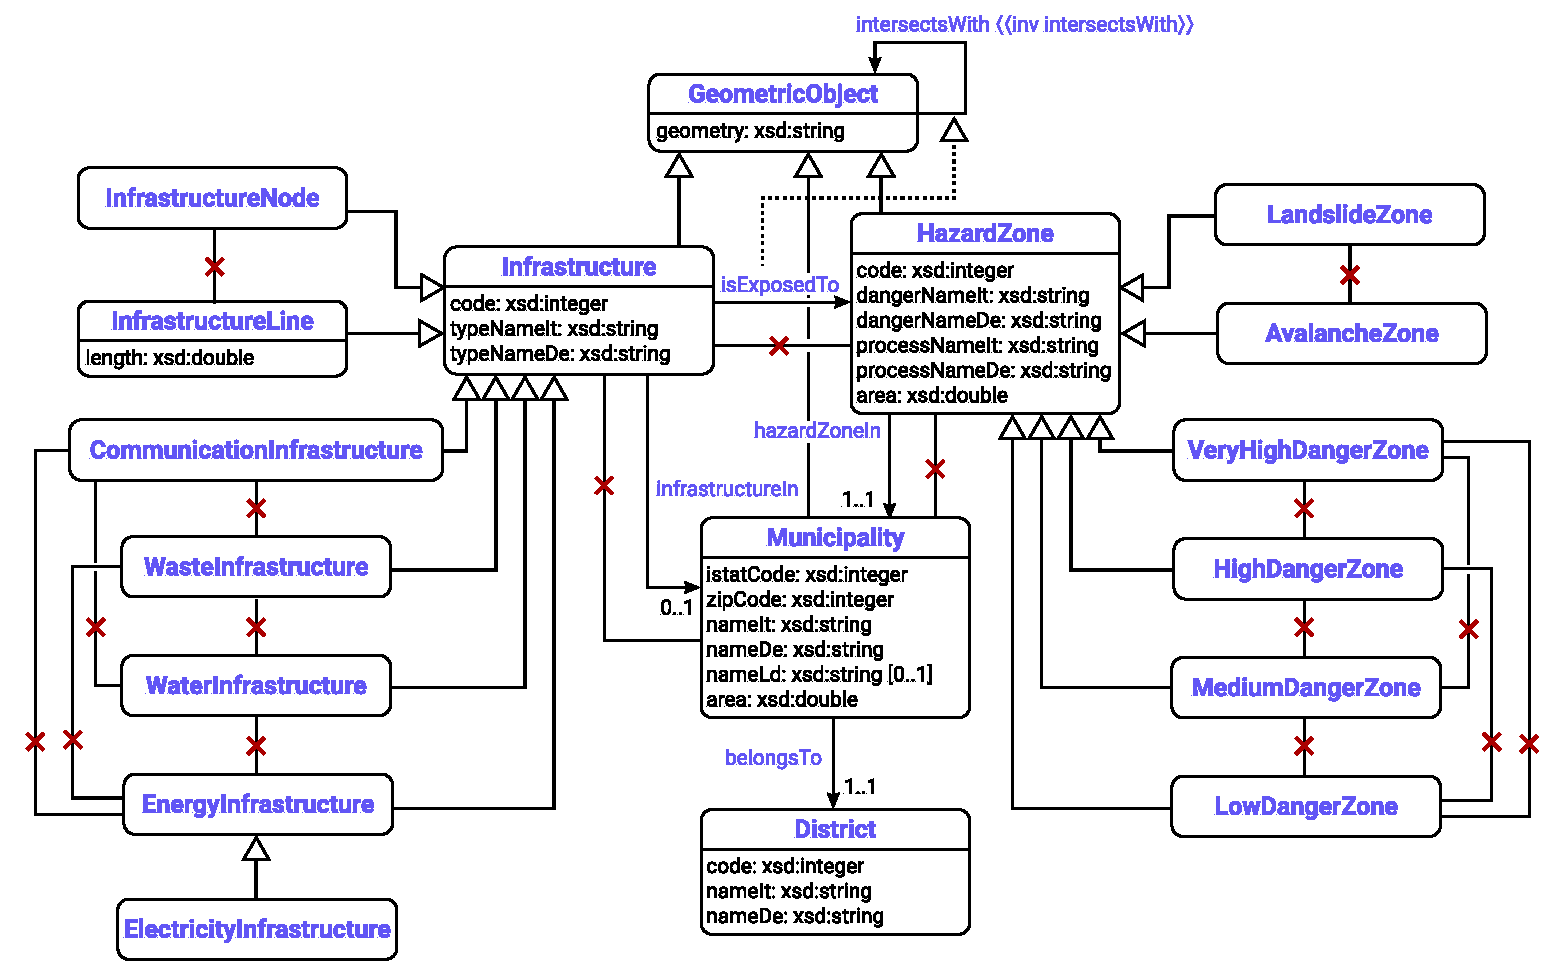
\includegraphics[width=0.9\linewidth]{figures/ontology.pdf}};
  \end{tikzpicture}
  \titlepage
\end{frame}

\begin{frame}
\frametitle{Introduction}
  \begin{items}
    \begin{oitem}{\litem}
      Problem: {\footnotesize Track poses of multiple people in videos across multiple views.}
    \end{oitem}
    \begin{oitem}{\litem}
      Given: \\
      \sitem {\footnotesize Multiple synchronously recorded video sequences containing multiple people.} \\
      \sitem {\footnotesize Camera calibration parameters, including extrinsics, intrinsic and distortion.}
    \end{oitem}
    \begin{oitem}{\litem}
      Output: \\
      \sitem {\footnotesize 3D coordinates of skeletal joints for each subject over time.}
    \end{oitem}
  \end{items}
\end{frame}

\begin{frame}
\frametitle{Conclusion}
  \begin{items}
    \begin{oitem}{\litem}
      Summary: \\
      \sitem {\footnotesize Implemented an EKF framework that merges multi-view observations.} \\
      \sitem {\footnotesize Incorporated skeletal length consistency constraints.} \\
      \sitem {\footnotesize Implemented simple learning of parameters from data.} \\
      \sitem {\footnotesize Analyzed performance across different system configuration.}
    \end{oitem}
    \begin{oitem}{\litem}
      Limitations: \\
      \sitem {\footnotesize Still struggles significantly with occlusions.} \\
      \sitem {\footnotesize Running 2D pose estimation remains a performance bottleneck.}
    \end{oitem}
    \begin{oitem}{\litem}
      Possible Future Improvements: \\
      \sitem {\footnotesize Add more constraints that force other known properties.}\\
      \sitem {\footnotesize Find more stable learning methods for the Kalman filter parameters.} \\
      \sitem {\footnotesize Use of a particle filter with occlusion aware likelihood.}
    \end{oitem}
  \end{items}
\end{frame}


{
\setbeamercolor{background canvas}{bg=black}
\begin{frame}[plain]{}
\end{frame}
}

\end{document}
